\documentclass[12pt,a4paper]{article}
\usepackage[utf8]{inputenc}
\usepackage{amsmath}
\usepackage{amsfonts}
\usepackage{amssymb}
\usepackage[brazil]{babel}
\usepackage{indentfirst}
\usepackage{url}
\usepackage{float}
\usepackage{color}
%%%%%%%%%%Codigos para o JAVA%%%%%%%%%%%%%%%%%%%%%%%%%%%%%%%%
\definecolor{pblue}{rgb}{0.13,0.13,1}
\definecolor{pgreen}{rgb}{0,0.5,0}
\definecolor{pred}{rgb}{0.9,0,0}
\definecolor{pgrey}{rgb}{0.46,0.45,0.48}
\usepackage{listings}
\lstset{language=PHP,
  showspaces=false,
  showtabs=false,
  breaklines=true,
  showstringspaces=false,
  breakatwhitespace=true,
  commentstyle=\color{pgreen},
  keywordstyle=\color{pblue},
  stringstyle=\color{pred},
  basicstyle=\ttfamily,
  moredelim=[il][\textcolor{pgrey}]{\$\$},
  moredelim=[is][\textcolor{pgrey}]{\%\%}{\%\%}
}
\lstdefinestyle{LaTeX}{
  language={[LaTeX]TeX},
  basicstyle=\ttfamily\small, 
  identifierstyle=\color{black}, 
  keywordstyle=\color{blue}, 
  commentstyle=\color{red}, 
  extendedchars=true, 
  showspaces=false, 
  showstringspaces=false, 
  numbers=none,
  breaklines=true,
  backgroundcolor=\color{yellow!20}, 
  breakautoindent=true, 
  captionpos=b,
  xleftmargin=0pt,
  frame=none,
  rframe={},
}
%%%%%%%%%%%%%%%%%%%%%%%%%%%%%%%%Fim codigo JAVA%%%%%%%%%%%%%%
%%%%%%%%%%%Codigo geral%%%%%%%%%%%%%%%%%%%%%%%%%%%%%%%%%%%%%%
\definecolor{mygreen}{rgb}{0,0.6,0}
\definecolor{mygray}{rgb}{0.5,0.5,0.5}
\definecolor{mymauve}{rgb}{0.58,0,0.82}
\lstset{ %
  backgroundcolor=\color{white},   % choose the background color; you must add \usepackage{color} or \usepackage{xcolor}; should come as last argument
  basicstyle=\footnotesize,        % the size of the fonts that are used for the code
  breakatwhitespace=false,         % sets if automatic breaks should only happen at whitespace
  breaklines=true,                 % sets automatic line breaking
  captionpos=b,                    % sets the caption-position to bottom
  commentstyle=\color{mygreen},    % comment style
  deletekeywords={...},            % if you want to delete keywords from the given language
  escapeinside={\%*}{*)},          % if you want to add LaTeX within your code
  extendedchars=true,              % lets you use non-ASCII characters; for 8-bits encodings only, does not work with UTF-8
  frame=single,                    % adds a frame around the code
  keepspaces=true,                 % keeps spaces in text, useful for keeping indentation of code (possibly needs columns=flexible)
  keywordstyle=\color{blue},       % keyword style
  language=Octave,                 % the language of the code
  morekeywords={*,...},            % if you want to add more keywords to the set
  numbers=left,                    % where to put the line-numbers; possible values are (none, left, right)
  numbersep=5pt,                   % how far the line-numbers are from the code
  numberstyle=\tiny\color{mygray}, % the style that is used for the line-numbers
  rulecolor=\color{black},         % if not set, the frame-color may be changed on line-breaks within not-black text (e.g. comments (green here))
  showspaces=false,                % show spaces everywhere adding particular underscores; it overrides 'showstringspaces'
  showstringspaces=false,          % underline spaces within strings only
  showtabs=false,                  % show tabs within strings adding particular underscores
  stepnumber=1,                    % the step between two line-numbers. If it's 1, each line will be numbered
  stringstyle=\color{mymauve},     % string literal style
  tabsize=2,                       % sets default tabsize to 2 spaces
  title=\lstname                   % show the filename of files included with \lstinputlisting; also try caption instead of title
}
%%%%%%%%%%%%%%%%%%%%%%%%%%%%%%%%Fim codigo geral%%%%%%%%%%%%%
\RequirePackage{graphicx}
\title{Banco de Dados de anúncios}
\author{Andrey Ribeiro \and Jeferson Rossini\and Wesley Morais\and Marcos Arriel\and Jonathan Sousa}
 
\usepackage[left=3cm,right=3cm,top=2cm,bottom=2cm]{geometry}
\begin{document}
\begin{titlepage}
\begin{center}
\begin{figure}[htb]
                
                \label{figura:LogoIF}
        
                \centering
                
\includegraphics[width=6cm]{recursos/imagens/logo.png} 
\end{figure}
Instituto Federal Goiano - Campus Ceres\\
Bacharelado em Sistemas de Informação\\
Prof. Me. Ronneesley Moura Teles\\\vspace{0.5cm}
Andrey Ribeiro \\
Jeferson Rossini\\
Wesley Morais\\
Marcos Arriel\\
Jonathan Sousa\\
\vspace{5.0cm}
\textit{\textbf{\Large{Banco de Dados de anúncios}}}\\\vspace{0.5cm}
\vspace{9.5cm}
\end{center}
\end{titlepage}
\tableofcontents
\newpage
\begin{center}
\textbf{\Large{Banco de Dados de anúncios }}\\\vspace{0.5cm}
\end{center}
\section{Introdução}
Este artigo contém uma modelagem e uma estrutura de armazenamento de dados para um sistema de controle de resultados de uma campanha de publicidade. Com a contrução de um sistema que gerência e controla todos os resultados de uma campanha de publicidade, tais como região em que deseja anunciar, público, quantidade de visualizações do anuncio ou cliques neles, formas de pagamento, crédito prévio para o anúncio, podendo ser adaptado para diversos outros projetos que necessitem de um controle e medição de resultados publicitários.

\section{DER}

\begin{figure}[h]
\centering
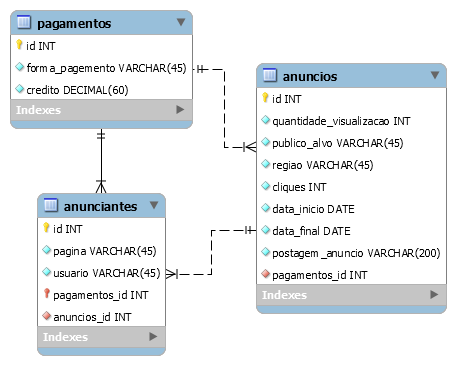
\includegraphics[width=15cm]{recursos/DER.png}
\label{4}
\caption{DER do Banco da Dados}
\end{figure}

\section{Como funciona?}
Cada anunciantes tem sua página e seu usuário, com isso ele pode criar um anuncio que conta a quantidade de visualizações, o publico alvo, a regiao, os cliques, a data de início e fim e a postagem que foi anunciada, além disso conta com a forma de pagamento e o crédito prévio para propagandas.

\subsection{anuncio.sql}
SQL do Banco de Dados.
\lstinputlisting{recursos/anuncio.sql}

\subsection{inserts.sql}
Inserts do Banco de Dados
\lstinputlisting{recursos/inserts.sql}

\subsection{view.sql}
View utilizadas no Banco de Dados
\lstinputlisting{recursos/views.sql}
\end{document}
%Modelo de código para inserir figura
%\begin{figure}[h]
%\centering
%
\includegraphics[width=15cm]{logo.png}
%\label{4}
%\caption{Fonte:http://...; Acesso em 06/11/2017}
%\end{figure}